%----------------------------------------------------------------------------
\chapter{Időzített automata generátor}
%----------------------------------------------------------------------------

%----------------------------------------------------------------------------
\section{Az automata generátor célja}
%----------------------------------------------------------------------------

A diplomatervezés során elkészített automata generátort kibővítettem úgy, hogy támogassa a TPSC elemekhez tartozó automata minták generálását. Bemenetként egy TPSC scenario szöveges leírását kapja meg amiből a minta alapú módszerrel generál egy TA automatát.

A 13. ábrán látható, hogy a monitor generátor támogatja az alt, par és loop operátorokat tartalmazó TPSC-khez tartozó TA-k generálását is. Továbbá a generátor képes az üzenet paraméterek kezelésére. Például az alt operátor feltételét képes feldolgozni és azt elhelyezni a generált automata megfelelő élén.

%----------------------------------------------------------------------------
\section{Az automata generátor megvalósítása}
%----------------------------------------------------------------------------
A generátorhoz az Xtend technológiát használtam. Minden egyes TPSC üzenethez legenerálja a hozzá tartozó minta automatát, majd elvégzi azok összecsatolását.

Az időzített automaták generálásához egy adatstruktúrát definiáltam, amely a következő Java osztályokból áll:
\begin{itemize}
    \item State
    \item StateType
    \item Transition
    \item Automaton
    \item Specification
\end{itemize}

A 14. ábrán látható az adatstruktúra UML osztály diagramja.

\begin{figure}[h!]
    \centering
    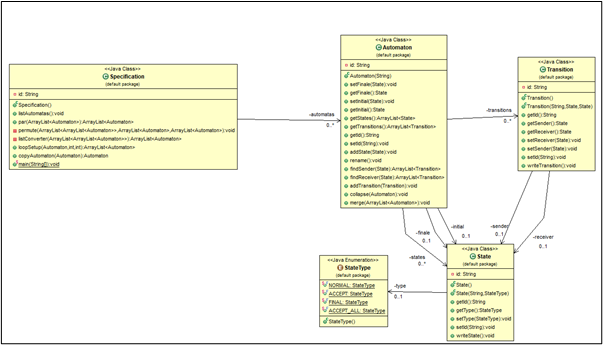
\includegraphics[width=150mm, keepaspectratio]{figures/13abra.png}
    \caption{Az adatstruktúra UML osztály diagramja.}
\end{figure}

Az automatában lévő állapotok implementációja a State osztályban található. Két attribútuma van: id(String), a címkéje tárolására, és type(StateType), az állapot típusa.

Az állapot típusának a megadására a StateType enum osztályt definiáltam. NORMAL, ACCEPT, FINAL értékeket lehet benne eltárolni. Az átmenetek implementációjáért felelős osztály a Transition. Három tag változója van: id(String) az üzenet, sender(State), a feladó állapot, és receiver(State) a fogadó állapot.

Az időzített automata implementációja az Automaton osztályban található. Itt tároljuk az automatában lévő állapotokat és a köztük lévő átmeneteket egy-egy listában. Az Automaton osztály addState(State) és addTransition(Transition) függvényeivel lehet új állapotot és átmenetet hozzáadni az automatához, a collapse(Automaton) függvényével pedig két automatát egyesíteni. Ezt a függvényt használtam az implementációban a minta automaták egyesítésére. Ezen kívül az osztálynak van egy merge(ArrayList<Automaton>) függvénye. Ez az előző fejezetben definiált merge függvény implementációja.

A Specification osztály feladata, hogy összeállítsa a szöveges leírásban specifikált TPSC scenariohoz tartozó időzített automatát. Ezt követően az automata Never Claim leírását egy .txt kiterjesztésű fájlba írja.

%----------------------------------------------------------------------------
\section{Minta példa}
%----------------------------------------------------------------------------

\begin{figure}[h!]
    \centering
    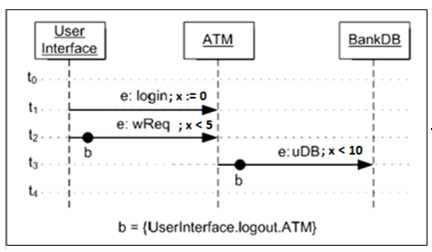
\includegraphics[width=150mm, keepaspectratio]{figures/14abra.png}
    \caption{Példa TPSC diagram.}
\end{figure}

\begin{lstlisting}[language=java,frame=single, float=h!, caption={TPSC scenario szöveges leírása.},captionpos=b]
specification Bank {
	object User_Interface ui;
	object ATM atm;
	object BankDB db;

	clock x;

	constraint b {
		message logout() ui -> atm;
	}

	scenario transaction {
		message login() ui -> atm reset x;
		message wReq() required ui -> atm pastConstraint {b, x < 1} clockConstraint {x < 5};
		message uDB() atm -> db clockConstraint {x < 10};
	}
}
\end{lstlisting}

\begin{lstlisting}[language=java,frame=single, float=h!, caption={Generált időzített automata never claim formátumban.},captionpos=b]
never{ /*transactionMonitor*/
T0_init:
 if
 :: (!(ui.login().atm); ) -> goto T0_init
 :: (ui.login().atm; x = 0) -> goto T0_q1
 fi;
T0_q1:
 if
 :: (!(ui.wReq().atm); x < 5 & !(ui.logout().atm); x < 1)) -> goto T0_q1
 :: (ui.wReq().atm; x < 5) -> goto T0_q3
 :: ((!(!(ui.logout().atm); x < 1); x < 5) || (ui.wReq().atm; )) || (1, x >= 5))) -> goto accept_q2
 fi;
accept_q2:
 if
 fi;
T0_q3:
 if
 :: (!(atm.uDB().db); x < 10;) -> goto T0_q3
 :: (atm.uDB().db; x < 10;) -> goto T0_q4
 fi;
T0_q4:
 if
 fi;
}
\end{lstlisting}

A fenti 14., 15. és 16. ábrákon látható, hogy a generátor milyen időzített automatát generál a megadott TPSC scenario-ból.